%_______________________________________________________________________________
%class
%_______________________________________________________________________________
%\documentclass[a4paper,11pt,onecolumn,final,german,openbib]{scrbook}
\documentclass[a4paper,10pt,oneside,final,german,openbib,pdftex,titlepage]{scrbook}
%_______________________________________________________________________________
% page borders
%_______________________________________________________________________________
\addtolength{\headheight}{2cm}
%\addtolength{\topmargin}{2cm}
\setlength{\oddsidemargin}{1.0cm}
\setlength{\evensidemargin}{0.5cm}
\setlength{\textwidth}{14.3cm}
\setlength{\parindent}{0mm}

%_______________________________________________________________________________
% packages
%_______________________________________________________________________________
\usepackage{german}
\usepackage{amsmath, amssymb}
\usepackage[utf8]{inputenc}
\usepackage{graphicx}
\usepackage{enumerate}
\usepackage{multirow}
\usepackage{subfigure}
\usepackage{dsfont}
\usepackage{slashed}
\usepackage{textcomp}
\usepackage{url}
\usepackage{mathtools}
\usepackage{chngcntr}
\usepackage{MnSymbol}
\usepackage{wasysym}
\usepackage{amsmath}
\usepackage{amssymb}
\usepackage{amsthm}
\usepackage{graphicx}
%\usepackage{MnSymbol}
\usepackage{hyperref}
\usepackage{setspace}
\usepackage{framed} 
\usepackage{xcolor} 
\usepackage{blindtext}
\usepackage{float}
\usepackage{tikz}
\usetikzlibrary{matrix}
%_______________________________________________________________________________
% bold fonts for headings
%_______________________________________________________________________________
\font\afont=cmssbx10 scaled \magstep5     % for the title
\font\bfont=cmssbx10 scaled \magstep4     % for chapter headings
\font\cfont=cmssbx10 scaled \magstep3
\font\dfont=cmssbx10 scaled \magstep2     % for section headings and author name
\font\efont=cmssbx10 scaled \magstephalf

%_______________________________________________________________________________
% index depth
%_______________________________________________________________________________
\setcounter{secnumdepth}{3}
\setcounter{tocdepth}{3}

%_______________________________________________________________________________
% new commands
%_______________________________________________________________________________
\newcommand{\demi}{\frac{1}{2}}

%_______________________________________________________________________________
% renewed commands
%_______________________________________________________________________________
% \renewcommand{\topfraction}{1.}       % this is important for figure placement
% \renewcommand{\bottomfraction}{1.}
\makeatletter
\renewcommand\paragraph{\@startsection{paragraph}{4}{\z@}%
  {-3.25ex\@plus -1ex \@minus -.2ex}%
  {1.5ex \@plus .2ex}%
  {\normalfont\normalsize\bfseries}
}
\makeatother



%_______________________________________________________________________________
% special words, hyphenation
%_______________________________________________________________________________
\hyphenation{Ba-che-lor-ar-beit}

\pagestyle{empty}
\pagestyle{headings}
%for changing the style on a specific page use \thispagestyle{e.g., empty}


\renewcommand*{\chapterheadstartvskip}{\vspace*{-25pt}}	
%\renewcommand*{\chapterheadstartvskip}{\vspace*{.0\baselineskip}}%
% Abstand einstellen


%_______________________________________________________________________________
%_______________________________________________________________________________

\usepackage{scrpage2} 
%\deftripstyle{default}{}{\leftmark\ -- \rightmark}{}{}\thepage{}{} 
%\pagestyle{default} 
\automark[section]{section}



\begin{document}

\colorlet{shadecolor}{gray!25} 

\pagenumbering{roman}
\linespread{0.9}

%_______________________________________________________________________________
\begin{titlepage}

  \vspace*{6mm}
  \begin{center}
     {\afont Stable Fluids}
     \\[3.5cm]
     {\large by}
     \\[3.5cm]
     {\dfont Lukas Polthier, Johannes von Lindheim}\\
     {based on Stam, 1999}
     \\[2cm]
     {\large Scientific Visualization, winter 15/16\/\\
}
   \end{center}
   \vfill
   Supervisor: Prof. Dr. Konrad Polthier\\	
   %Zweitgutachter: n.n.  \\
   \vfill
   
   
\end{titlepage}

\newpage
\mbox{}
\thispagestyle{empty}

\newpage
\thispagestyle{empty}
We hereby declare that this article is based on our work, unless stated otherwise. No other person’s work has been used without due acknowledgement in this thesis. All references and verbatim extracts have been quoted, and all sources of information have been specifically acknowledged.
\\
\\[3.5cm] 
Berlin, \today
\vfill
\noindent 
Lukas Polthier\\
Johannes von Lindheim\\
Institut f\"ur Mathematik\\
Arnimallee 6\\
Freie Universit\"at Berlin\\
14195 Berlin\\
{\tt info@lukas-polthier.de\\
\tt jovoli@gmx.de}

%_______________________________________________________________________________
\thispagestyle{empty}
\renewcommand\contentsname{Table of Contents}
\thispagestyle{empty}
\renewcommand\figurename{Figure}
\renewcommand\tablename{Tabelle}
\thispagestyle{empty}
\tableofcontents
\thispagestyle{empty}
\clearpage
\thispagestyle{empty}

\mainmatter
\sloppy

\newtheoremstyle{test333}% name
    {\topsep}             % Space above
    {5pt}             % Space below
    {\itshape}         % Body font
    {\parindent}       % Indent amount (empty = no indent, \parindent = para indent)
    {\bfseries}        % Thm head font
    {:}                % Punctuation after thm head
    {.5em}             % Space after thm head: " " = normal interword space; \newline = linebreak
    {}                 % Thm head spec (can be left empty, meaning `normal')

\theoremstyle{test333}
\newtheorem{test333}{TEST}
\newtheorem{thm}{Theorem}


\theoremstyle{theorem}% default
\newtheorem{Lem}[thm]{Lemma}
\newtheorem{Cor}[thm]{Corollary}
\newtheorem{Def}[thm]{Definition}

\theoremstyle{definition}
\newtheorem{Rem}[thm]{Remark}
\newtheorem{State}[subsection]{\#}



\makeatletter
\g@addto@macro{\thm@space@setup}{\thm@headpunct{:}}
\makeatother

%_______________________________________________________________________________
\setcounter{chapter}{-1}
\chapter{Abstract}
\chapter{Introduction}

The concept of this solver is based on \cite{Stam}. The method of solution has been implemented in this article.
The program runs in the framework of JavaView \cite{JavaView}.

We added\\
 ->Colors\\
 ->Fotoimport\\
 ->nice user interface\\
 ->Insertion in the framework of JavaView.
 
\chapter{Mathematical Modelling} \label{Section:Mathematical Modelling}

\section{Basic Equations}
Let $\Omega \subset \mathbb{R}^2$ be the domain of interest, e.g. $\Omega = (0,1)^2$. Now let $u \in C^2(\mathbb{R} \times \Omega,\mathbb{R}^2)$ denote the velocity vector field and $p\in C^2(\mathbb{R} \times \Omega,\mathbb{R})$ denote the pressure field. Both fields depend on the time $t\in \mathbb{R}$ and the position in space $x\in \Omega$. The evolution of these fields is given by the Navier-Stokes equations
\begin{align}
	&\text{div } u = 0 \label{NavierStokes1}
	\\
	&\frac{\partial u}{\partial t} = - (u \cdot \nabla)u - \frac{1}{\rho}\nabla p + \nu \Delta u + f, \label{NavierStokes2}
\end{align}
where $\nu, \rho$ are constants that determine the viscosity of the fluid and the density respectively.
In $\mathbb{R}^2$, equation \ref{NavierStokes2} can be written out as
\begin{align*}
	\left( \begin{matrix}
	\frac{\partial u_1}{\partial t} \\ \frac{\partial u_2}{\partial t}
	\end{matrix} \right) = - \left(\begin{matrix}
	u_1 \frac{\partial u_1}{\partial x_1} + u_2 \frac{\partial u_1}{\partial x_2} \\ u_1 \frac{\partial u_2}{\partial x_1} + u_2 \frac{\partial u_2}{\partial x_2}
	\end{matrix} \right)  - \frac{1}{\rho} \left( \begin{matrix}
	\frac{\partial p}{\partial x_1} \\ \frac{\partial p}{\partial x_2}
\end{matrix}\right)	 + \nu \left( \begin{matrix}
	\frac{\partial^2 u_1}{\partial x_1^2} + \frac{\partial^2 u_1}{\partial x_2^2} \\ \frac{\partial^2 u_2}{\partial x_1^2} + \frac{\partial^2 u_2}{\partial x_2^2}
	\end{matrix} \right) + \left( \begin{matrix}
	f_1 \\ f_2
	\end{matrix} \right).
\end{align*}
The pressure and velocity field that appear in the Navier-Stokes equations, are related. By combining equation \ref{NavierStokes1} and \ref{NavierStokes2} we obtain a singe equation as follows.\\

By the Helmholtz-Hodge decomposition theorem we have that any vector field $w = u + \nabla q + \text{res}$ uniquely decomposes into a divergence-free part $u$, a gradient field $\nabla q$ and a residual term depending on the genus of the surface. In our case, the residual term vanishes.\\

Let $P : C^2(\Omega,\mathbb{R}^2) \rightarrow \{f\in C^2(\Omega, \mathbb{R}^2), \text{div} f = 0\}$ denote the projection operator onto the divergence free part. Obviously, the operator $P$ is implicitly defined by 
\begin{align}
	\text{div } w = \Delta q. \label{Poisson-1}
\end{align}
With Neumann boundary condition ($\frac{\partial q}{\partial n} = 0$ on $\partial \Omega$, $n$ is the outward normal), equation \ref{Poisson-1} is a Poisson equation. Let $q$ denote the solution, then $P$ is defined by $Pw = w - \nabla q$. 
If we now apply $P$ to both sides of \ref{NavierStokes2}, the Navier-Stokes equation compress into our fundamental equation \ref{FundamentalEquation}.
\begin{align}
	\frac{\partial u}{\partial t} = P \left(- (u \cdot \nabla)u - \frac{1}{\rho}\nabla p + \nu \Delta u + f \right) \label{FundamentalEquation}
\end{align}
\section{Method of Solution and Discretization}
Equation \ref{FundamentalEquation} consists of four parts, the \textbf{add force} term $f$, the \textbf{advection} term $(u\cdot \nabla )u$, the \textbf{diffusion} term $\nu \Delta u$ and the \textbf{projection} operator $P$. The equation is solved from an initial state $u^0 = u(0,x)$. Both time and space are discretized with time step $\Delta T$ and some equidistant grid points of distance $h= \frac{1}{n}$.
Each of the four terms in equation \ref{FundamentalEquation} is applied successively to the initial state $u^0 \in C^2(\Omega,\mathbb{R})$. The general procedure is
\begin{align*}
	u^0 ~\overset{\text{add force}}{\longrightarrow}~ u^1 ~ \overset{\text{advect}}{\longrightarrow}~ u^2 ~\overset{\text{diffuse}}{\longrightarrow} ~u^3~ \overset{\text{project}}{\longrightarrow} ~u^4
\end{align*}
The solution at time $t+\Delta t$ is then given by $u(x,t+\Delta t) = u^4(x)$.
\subsection{Add force}
The add force step incorporates additional force by the user, or buoyancy force due to uplift of lighter or hotter gases resp. downlift of heavier or cooler gases.
\begin{align*}
	u^1(x) = u^0(x) + \Delta t~ f(t,x)
\end{align*}
The buoyancy force is computed using Archimedes' principle. In a simplified approach, heaviness is equal to the density of the smoke. After computing the average temperature of the fluid, the upward force is determined for each pixel separately depending on the difference with respect to the average temperature.\\

[tba] exact formula of buoyancy force [tba]
\subsection{Advect}
The advect step accounts for the advection or convection of the fluid itself, i.e. this step lets the fluid \grqq flow\grqq ~or move a little according to its own speed.
The advection step is fundamental to this particular fluid solver. The design of the advection solving process is the reason why this method is called \glqq Stable\grqq ~Fluids, as this solver will never \grqq  blow up\grqq , independent of the size of the time step $\Delta t$. 

The method can be understood intuitively: All particles in the fluid are moved by the velocity of the fluid itself. To obtain the velocity at the point $x$ at time $t + \Delta t$ we backtrace the the point $x$ through the velocity field at time $t$. This defines a path $p: (-\delta,\delta) \times \Omega \rightarrow \Omega$ corresponding to a streamline of the fluid. The velocity $u^2(x)$ is the set to be the velocity of $u^1(p(-\Delta t,x))$ at the previous time step:
\begin{align*}
	u^2(x) = u^1(p(-\Delta t,x)).
\end{align*}
[tba] include a figure that illustrates the approach. [tba]
[tba] include a comparison to other solvers of the advect step. [tba]
\subsection{Diffuse}
This step solves the diffusion of the fluid itself, i.e. the \grqq friction\grqq ~between parts of the fluid with different velocity. This effect is equivalent to the diffusion equation 
\begin{align}
	\frac{\partial u^2}{\partial t} = \nu \Delta u^2. \label{Diffusion}
\end{align}
The most straightforward way would be to discretize the Laplacian and solve the resulting sparse linear system. However, this approach is unstable when the viscosity is large. For our implicit approach we proceed by approximating $\frac{\partial u}{\partial t}$ with the backward difference quotient:
\begin{align}
	\frac{u(t+\Delta t,x) - u(t,x)}{\Delta t} = \nu \Delta u(t-\Delta t,x) \nonumber
	\shortintertext{Finally, this yields}
	(I - \nu \Delta t) u^3(x) = u^2(x). \label{Diffusion2}
\end{align}
We now discretize \ref{Diffusion2} using a finite difference method and obtain
\begin{equation}
	(\begin{tikzpicture}[baseline=(current bounding box.center)]
		\matrix (m) [matrix of math nodes,nodes in empty cells,right 	delimiter={]},left delimiter={[} ]{
		1  &  &   &  & &   \\
	  	& & & & &  \\
	 	& & & & &    \\
	   	& & & & &   \\
	  	& & & & &  \\
	 	& & &  &  & 1\\
		} ;
		\draw[loosely dotted] (m-1-1)-- (m-6-6);
	\end{tikzpicture} - \begin{tikzpicture}[baseline=(current bounding box.center)]
	\matrix (m) [matrix of math nodes,nodes in empty cells,right delimiter={]},left delimiter={[} ] {
		-4  & 1 &   & 1 & &   \\
		 1 & & & & &  \\
		 & & & & & 1   \\
		  1 & & & & &   \\
		  & & & & & 1 \\
		 & & 1 &  & 1 & -4\\
		} ;
		\draw[loosely dotted] (m-1-1)-- (m-6-6);
		\draw[loosely dotted] (m-1-2)-- (m-5-6);
		\draw[loosely dotted] (m-2-1)-- (m-6-5);
		\draw[loosely dotted] (m-4-1)-- (m-6-3);
		\draw[loosely dotted] (m-1-4)-- (m-3-6);
	\end{tikzpicture} ~\nu\frac{\Delta t}{h^2} )u^3 = u^2.\label{Diffuse}
\end{equation}
The resulting square matrix has $n\cdot m$ rows and columns, where $n, m$ denote the number of pixels in the x- and y-axis respectively. Solving such a system can be done efficiently by iterative schemes, e.g. Gauß-Seidel.\\

[tba] make formatting nice, i.e. bigger brackets and identity bigger [tba]\\

\subsection{Project}
The last step makes the vectorfield mass preserving, i.e. divergence free. We already discussed in the derivation of our fundamental equation that the projection is obtained by solving
\begin{align*}
	\text{div }u = \Delta q.
\end{align*}
When discretized, this equation becomes
\begin{equation}
\frac{1}{2h}
	\begin{tikzpicture}[baseline=(current bounding box.center)]
		\matrix (m) [matrix of math nodes,nodes in empty cells,right 	delimiter={]},left delimiter={[} ]{
		0 & 1 & & &   &   \\
	  	1 &   & & &   &   \\
	 	  &   & & &   &   \\
	   	  &   & & &   &   \\
	  	  &   & & &   & 1 \\
	 	  &   & & & 1 & 0 \\
		} ;
		\draw[loosely dotted] (m-1-1)-- (m-6-6);
		\draw[loosely dotted] (m-1-2)-- (m-5-6);
		\draw[loosely dotted] (m-2-1)-- (m-6-5);
	\end{tikzpicture} u^3_1 + \frac{1}{2h} \begin{tikzpicture}[baseline=(current bounding box.center)]
		\matrix (m) [matrix of math nodes,nodes in empty cells,right 	delimiter={]},left delimiter={[} ]{
		0  &  &   & 1 & &   \\
	  	& & & & &  \\
	 	& & & & & 1  \\
	   	1& & & & &   \\
	  	& & & & &  \\
	 	& & 1&  &  & 0\\
		} ;
		\draw[loosely dotted] (m-1-4)-- (m-3-6);
		\draw[loosely dotted] (m-4-1)-- (m-6-3);
		\draw[loosely dotted] (m-1-1)-- (m-6-6);
	\end{tikzpicture} u^3_2 = 
	\begin{tikzpicture}[baseline=(current bounding box.center)]
	\matrix (m) [matrix of math nodes,nodes in empty cells,right delimiter={]},left delimiter={[} ] {
		-4  & 1 &   & 1 & &   \\
		 1 & & & & &  \\
		 & & & & & 1   \\
		  1 & & & & &   \\
		  & & & & & 1 \\
		 & & 1 &  & 1 & -4\\
		} ;
		\draw[loosely dotted] (m-1-1)-- (m-6-6);
		\draw[loosely dotted] (m-1-2)-- (m-5-6);
		\draw[loosely dotted] (m-2-1)-- (m-6-5);
		\draw[loosely dotted] (m-4-1)-- (m-6-3);
		\draw[loosely dotted] (m-1-4)-- (m-3-6);
	\end{tikzpicture} ~q.\label{Project}
\end{equation}
As in equation \ref{Diffuse} we need to solve a sparse linear system.

\section{Moving substances through the Fluid}
Our solver enables us to compute the ambient fluid. However, we need to visualize the vector field. A substance, that is injected in the fluid and does not interact with it, will be advected by the vector field and diffuse at the same time. Let $d \in C^2(\mathbb{R}^+\times\Omega, \mathbb{R})$ denote the density field of such a substance. The evolution of this scalar field is given by
\begin{align}
	\frac{\partial d}{\partial t} = - u \cdot \nabla a + \kappa \Delta a - \alpha  a + S \label{Density}
\end{align}
where $\kappa$ is the diffusion constant, $\alpha$ the dissipation term and $S$ is a source term. The dissipation term, which will be dropped in our modelling, describes the effect that kinetic energy is converted in thermal energy. The diffusion constant determines the effect of diffusion, i.e. the effect that density \grqq interfuses\grqq ~with nearby density and the overall picture becomes \grqq  softer\grqq .\\

The terms in equation \ref{Density} are quite similar to the terms in our fundamental equation \ref{FundamentalEquation}. Thus the evolution of the density field can be computed analogously to the computation of the velocity field. In particular we need to perform the advect step and the diffuse step, which correspond to the movement of the density along the velocity field and the diffusion of the density itself.

\section{Vorticity Confinement}
For sufficiently number of grid points, the steps in the previous section \ref{Section:Mathematical Modelling} give the fluid a realistic behaviour, quite similar to the real life experience. In practice, computational power is limited and we have to use a relatively small number of grid points to provide real-time computation. It turns out that small scale details, in particular rotational turbulences are lost due to numerical dissipation.

The key idea of Vorticity Confinement is to add these details artificially in a way that the properties of a fluid are preserved and the effect of numerical dissipation is damped. In a follow-up paper \cite{Stam2}, Stam proposes this idea based on previous work of Steinhoff \cite{Steinhoff}.\\

The vorticity of a 3d vector field $u$ is defined as
\begin{align*}
	\omega = \nabla \times u,
\end{align*}
i.e. in our two dimensional case, we have
\begin{align*}
	\omega = \left( \begin{matrix}
	\frac{\partial}{\partial x_1} \\ \frac{\partial}{\partial x_2} \\ \frac{\partial}{\partial x_3}
	\end{matrix} \right) \times 
	\left( \begin{matrix}
	u^1 \\ u^2 \\ 0
	\end{matrix} \right) = \left( \begin{matrix}
	 0\\ 0 \\ \frac{\partial}{\partial x_1} u^2 - \frac{\partial}{\partial x_2} u^1 
	\end{matrix} \right).
\end{align*}
We identify $\omega$ with a 1d scalar field on $\Omega$. The vorticity measures the amount of small scale detail of the fluid. The normalized gradient of the absolute vorticity
\begin{align*}
	N = \frac{\nabla |\omega |}{|\nabla  |\omega ||}
\end{align*}
is a vector field on $\Omega$ that points from regions of low to high vorticity.\\
Finally the small scale detail is added as follows
\begin{align}
	f = \varepsilon h (N\times \omega ) = \left( \begin{matrix}
	N^1\\ N^2 \\0
	\end{matrix}  \right) \times \left( \begin{matrix} 0\\ 0\\ \omega \end{matrix} \right) = \left( \begin{matrix}
	N^2 \omega \\ -N^1 \omega \\ 0
	\end{matrix} \right). \label{VorticityConfinement}
\end{align}
Again in equation \ref{VorticityConfinement} we identify 2d vector fields with 3d vector fields that are constant in the with respect to the direction of the $x^3$-axis.
Here $\varepsilon >0$ is a factor that determines the effect of vorticity confinement. The dependence on $h$ gives that small scale detail is added proportional to the grid size, i.e. to the numerical dissipation. Hence the convergence of the solver is preserved.\\
In fact the construction provides that small scale detail is added, exactly where it is needed.

\begin{figure}[H]
 \centering
 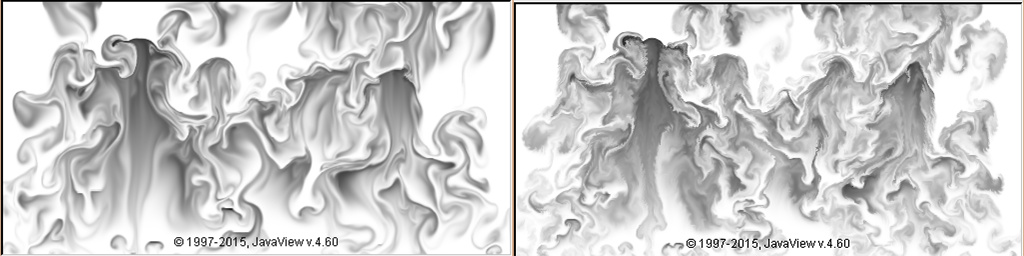
\includegraphics[scale=0.30]{images/Vorticity.png}
 \caption{The left picture shows the fluid solver without vorticity confinement, whereas the right picture shows the same setting with medium vorticity confinement. Both pictures where computed with the same grid size and initial configuration. One can see clearly how the left picture misses small scale rotational turbulences. The right picture provides a more gaseous behaviour of the fluid.}
 \label{VorticityOnOff}
\end{figure}

\section{Dependence on the Parameters}
The solver is compatible with a wide range of parameters. Thus we can simulate different kinds of fluids, depending on viscosity, buoyancy force, diffusion, etc.

\begin{figure}[H]
 \centering
 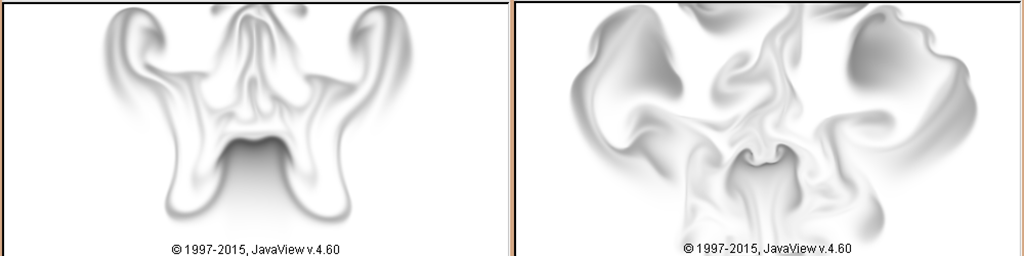
\includegraphics[scale=0.30]{images/Viscosity-2.png}
 \caption{The left picture shows a fluid with high viscosity, e.g. honey or very thick water. The right picture shows a more liquid fluid like thin water or some gas. The left picture preser [tba] end the sentence [tba] Both pictures where created with identical initial condition and vary only in the viscosity constant. In both pictures there is no vorticity confinement to emphasize the effect of viscosity.}
 \label{ViscosityOnOff}
\end{figure}

\begin{figure}[H]
 \centering
 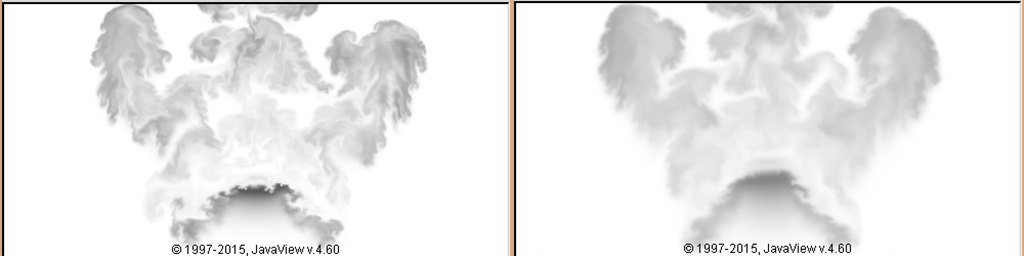
\includegraphics[scale=0.30]{images/Diffusion.png}
 \caption{In the left picture there is no diffusion, whereas in the right picture we can clearly see how diffusion influences the nature of the fluid. There are less details and the picture looks overall smoother. Again both simulations vary only in the effect of diffusion and are computed with the same resolution.}
 \label{ViscosityOnOff}
\end{figure}

\section{Colors and Fotoimport}
There are several ways to represent colors. One of the most common priciples are RGB or CMY color schemes. In the black and white solver there is only one density array which evolves according to the velocity field. To represent colors, we use three separate density fields, each one of them representing either cyan, magenta or yellow and evolving according to the same velocity field, i.e. the same \grqq ambient fluid\grqq.\\
We are now able to import picture, which behave like liquid or smoke, i.e. the picture can be manipulated interactively and behaves like the ambient fluid.\\
One can experiment with different kinds of buoyancy forces, e.g. only specific colors generate an uplift. However 

\chapter{Implementation and Framework}
We implemented our whole framework in the environment of JavaView. In the following, we want to show some features of our application, how they work and why we think they make sense for visualizing smoke.
%
\section{Capabilities of JavaView}
We want to give a brief overview over the features of JavaView that were used in the development of the project and also how they were used.
\begin{itemize}
\item To be able to show an image visualizing the smoke in the application, we use the common \texttt{PvDisplayIf} class. One can fix the camera over an x-y-coordinate system by selecting the correct camera: \texttt{m\_disp.selectCamera(PvCameraIf.CAMERA\_ORTHO\_XY)}. Then one can set the image one is manipulating as the background image by \texttt{m\_disp.setBackgroundImage(m\_image)}.
\item For handling mouse input, there are the two functions \texttt{pickInitial(PvPickEvent pickEvent)} and \texttt{dragCamera(PvCameraEvent cameraEvent)} which are invoked by JavaView, when the left resp. right mouse button is clicked. These methods were overwritten to add smoke resp. force. The mouse coordinates can be obtained from the corresponding events in the parameter list.
\item The parameters of the fluid solver (the \grqq mathematics object\grqq) and block size (see below) are controlled by sliders in the application. One is able to add these for types like \texttt{PuInteger} or \texttt{PuDouble} by for instance adding \texttt{m\_Project.m\_vorticityConf} to some \texttt{PsPanel} in the application.
\item Time can be handled by an animation, i.e. an instance of the class \texttt{PsAnimation}. Registering this animation in the project class' superclass makes JavaView invoke the method \texttt{setTime(PsTimeEvent timeEvent)} which was overwritten to call our \texttt{computeImage()}-function. To overcome the problem, that every animation has a maximum time, we are increasing the maximum by one timestep for every call of \texttt{setTime}.
\item When the user drags though the display with the left mouse button, the corresponding \texttt{PvPickEvent}s yield some loose points in the canvas. The class \texttt{PgBezierCurve} is used to connect them with spline curves, such that there is not only some bumps, but a whole continuous trace of smoke added in the cancas, like one would expect for instance from a pen. For details, see \ref{splinesChapter}.
\end{itemize}
%
\section{Splines}\label{splinesChapter}
As mentioned above, the user is able to \grqq draw\grqq~smoke with the left mouse button like with a pen, even though JavaView just provides a handful of input points. If we just would add smoke there, just some single pixels would be provided with some smoke.\\

\begin{figure}[H]
 \centering
 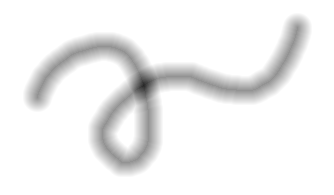
\includegraphics[scale=0.8]{images/SmokeTrace.png}
 \caption{Some smoke drawn into the display by the user with the mouse.}
 \label{SmokeTrace}
\end{figure}
To be able to achieve this, we connected the mouse input points from between two frames with a spline curve consisting of mostly cubic bezier curves or lower degree at the start or end where less information is available about the continuation of the curve. The resulting spline curve is $C^1$-continuous.\\

We also show the formula for the control points in the general case of cubic curves.
\begin{figure}[H]
 \centering
 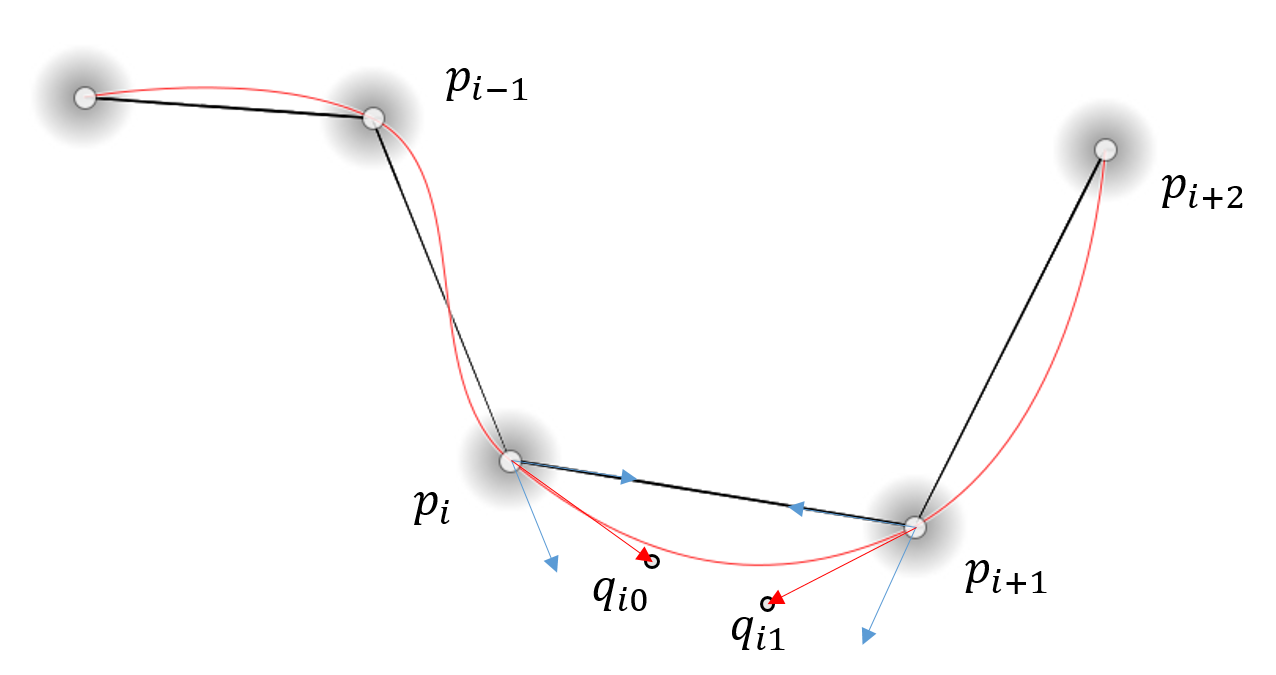
\includegraphics[scale=0.3]{images/SplinesScheme.png}
 \caption{Scheme how control points are computed.}
 \label{SplinesScheme}
\end{figure}
Then we compute the control points of the connecting cubic bezier curve to be
\begin{align*}
q_{i0} & = p_i + \alpha |p_i-p_{i+1}| \cdot \left((p_i-p_{i-1})^{\star} + (p_{i+1}-p_i)^{\star}\right)^{\star} \\
q_{i1} & = p_{i+1} + \alpha |p_i-p_{i+1}| \cdot \left((p_i-p_{i+1})^{\star} + (p_{i+1}-p_{i+2})^{\star}\right)^{\star}
\end{align*}
where $p^{\star}$ is a notation for $\frac{p}{|p|}$. In our case we chose $\alpha = \frac{2}{5}$. 
\section{Block-Size}
Since for a large enough canvas sizes interaction with the smoke in real time is not possible because of the large amount of computations, the user should be able to choose lower resolutions on the same canvas size to make the application run faster. The corresponding (larger) pixels are called \emph{blocks}.\\

If the user wants to change the size of a block, the color value of the new blocks are taken to be the average of the previous color of all pixels, that lie in that block.
%
%
%
\chapter{Results}
\chapter{Possible extensions}
\chapter{Outlook}

Bezier curves\\
Reference List\\
Blocksize\\
Capabilities of Javaview\\
Details vom Solver, Wie funktioniert ein Schritt genau? e.g. Beschreibe den Advect-Schritt detailliert (Pseudocode)\\
Physikalische Beschreibung der Navier-Stokes\\
Genaue Formel der buoyancy force\\
Bewertung der Results -> Was ist gut, was ist schlecht\\
Anleitung um hübsche Bilder zu generieren, Tutorial um den Solver zu verwenden\\
Verlgleich der einzelnen Schritte vom Solver mit alternativen Lösungsansätzen -> Warum ist der Solver STABLE\\
Darstellung der Farben mit Density-Arrays\\
Gauß-Seidel\\
Boundary Conditions\\
Abstract (Zusammenfassung)\\
Introduction (Einlietung, Historie.\\

%_______________________________________________________________________________
\begin{appendix}


%_______________________________________________________________________________
%\chapter{Reference list}
\renewcommand{\bibname}{\bfont Reference List} 
\bibliographystyle{h-physrev3}
\begin{thebibliography}{99}
%\cite{thepnews}

\bibitem{Alt}
H. Alt: ``Lineare Funktionalanalysis'', fifth edition, Springer, 2006.

\bibitem{Stam}
J. Stam: ``Stable Fluids'', Siggraph, 1999.

\bibitem{Stam2}
R. Fedkiw, J. Stam, H. W. Jensen: Visual Simulation of Smoke, Siggraph, 2001.

\bibitem{JavaView}
K. Polthier: JavaView, program refer to javaview.de.

\bibitem{Steinhoff}
J. Steinhoff, D. Underhill. Modification of the euler equations
for “vorticity confinement”: Application to the computation
of interacting vortex rings. Physics of Fluids, 6(8):2738–
2744, 1994.

\bibitem{Stoer1}
J. Stoer: ``Numerische Mathematik 1'', ninth edition, Springer, 2005.

\bibitem{StoerBulirsch2}
J. Stoer, R. Bulirsch: ``Numerische Mathematik 2'', fifth edition, Springer, 2005.

\end{thebibliography}
\end{appendix}

\end{document} 
        
        